\documentclass[pdftex,12pt,a4paper]{article}

\usepackage[utf8]{inputenc}
\usepackage[T1]{fontenc}
\usepackage[frenchb]{babel}
\usepackage{color}
\usepackage[usenames,dvipsnames,svgnames,table]{xcolor}
\usepackage{lmodern}
\usepackage{lastpage}
\usepackage[pdftex]{graphicx}
\usepackage{fancyhdr}
\usepackage{geometry}
\usepackage{url}
\usepackage[colorlinks=true,urlcolor=black,linkcolor=black]{hyperref}
\usepackage{fancyvrb}
\usepackage{multicol}
\usepackage[section]{placeins}
\usepackage{shorttoc}


\geometry{top=3cm, bottom=2.5cm, left=2cm, right=2cm}
\setcounter{tocdepth}{3}

%%%%%%%  VARIABLES     %%%%%%%%%%%%%%%%%%%%%%%%%%%%%%%%%%%%%
\newcommand{\docauthor}{
			Jeremy  \textsc{Bardon} \\
			Nicolas \textsc{Brondin} \\
			Adrien \textsc{Garandel} \\
            Maxime \textsc{Pauvert} \\
            David \textsc{Perrai} \\
            Anthony \textsc{Pena}           
 }
\newcommand{\doctitle}{Madjan}
%%%%%%%%%%%%%%%%%%%%%%%%%%%%%%%%%%%%%%%%%%%%%%%%%%%%%%%%%%%%

%%%%%%%   MAKE TITLE   %%%%%%%%%%%%%%%%%%%%%%%%%%%%%%%%%%%%%
\author{\docauthor}
\title{\doctitle}
\date{\today}
%%%%%%%%%%%%%%%%%%%%%%%%%%%%%%%%%%%%%%%%%%%%%%%%%%%%%%%%%%%%

%%%%%%  EN-TETE / PIED-PAGE %%%%%%%%%%%%%%%%%%%%%%%%%%%%%%%%
\pagestyle{fancy}
\fancyhead{}
\fancyfoot{}
\lhead{\leftmark}
\rhead{\doctitle}
\rfoot{\thepage/\pageref{LastPage}}
\lfoot{Concepts et outils de développement}
\renewcommand{\footrulewidth}{0.5pt}
\renewcommand{\headrulewidth}{0.5pt}
%%%%%%%%%%%%%%%%%%%%%%%%%%%%%%%%%%%%%%%%%%%%%%%%%%%%%%%%%%%%

\newcommand{\name}[1]{\textsc{#1}}
\newcommand{\commande}[1]{\texttt{#1}}

\fvset{frame=single,fontsize=\scriptsize,xleftmargin=2cm,xrightmargin=2cm}

\renewcommand{\FrenchLabelItem}{\textbullet}

\newcommand{\HRule}{\rule{\linewidth}{0.5mm}}

%% commande pour la création de balise ouvrante et fermante xml avec un texte centrale
\newcommand{\balise}[2]{\texttt{%
\textbf{\textless#1\textgreater}%
#2%
\textbf{\textless/#1\textgreater}%
}}
%% commande pour la création d'une balise ouvrante et fermante avec un ou plusieurs paramètres
\newcommand{\bwithparam}[3]{\texttt{%
\textbf{\textless#1}#2\textbf{\textgreater}\\%
\hspace*{0.5cm} #3\\%
\textbf{\textless/#1\textgreater}%
}}

\setlength{\parskip}{1ex plus .8ex minus .8ex}
\setlength{\parindent}{.8em}
\linespread{1.3}
%%%%%%%%%%%%%%%%%%%%%%%%%%%%%%%%%%%%%%%%%%%%%%%%%%%%%%%%%%%%

\begin{document}

  \begin{titlepage}
    \begin{center}
      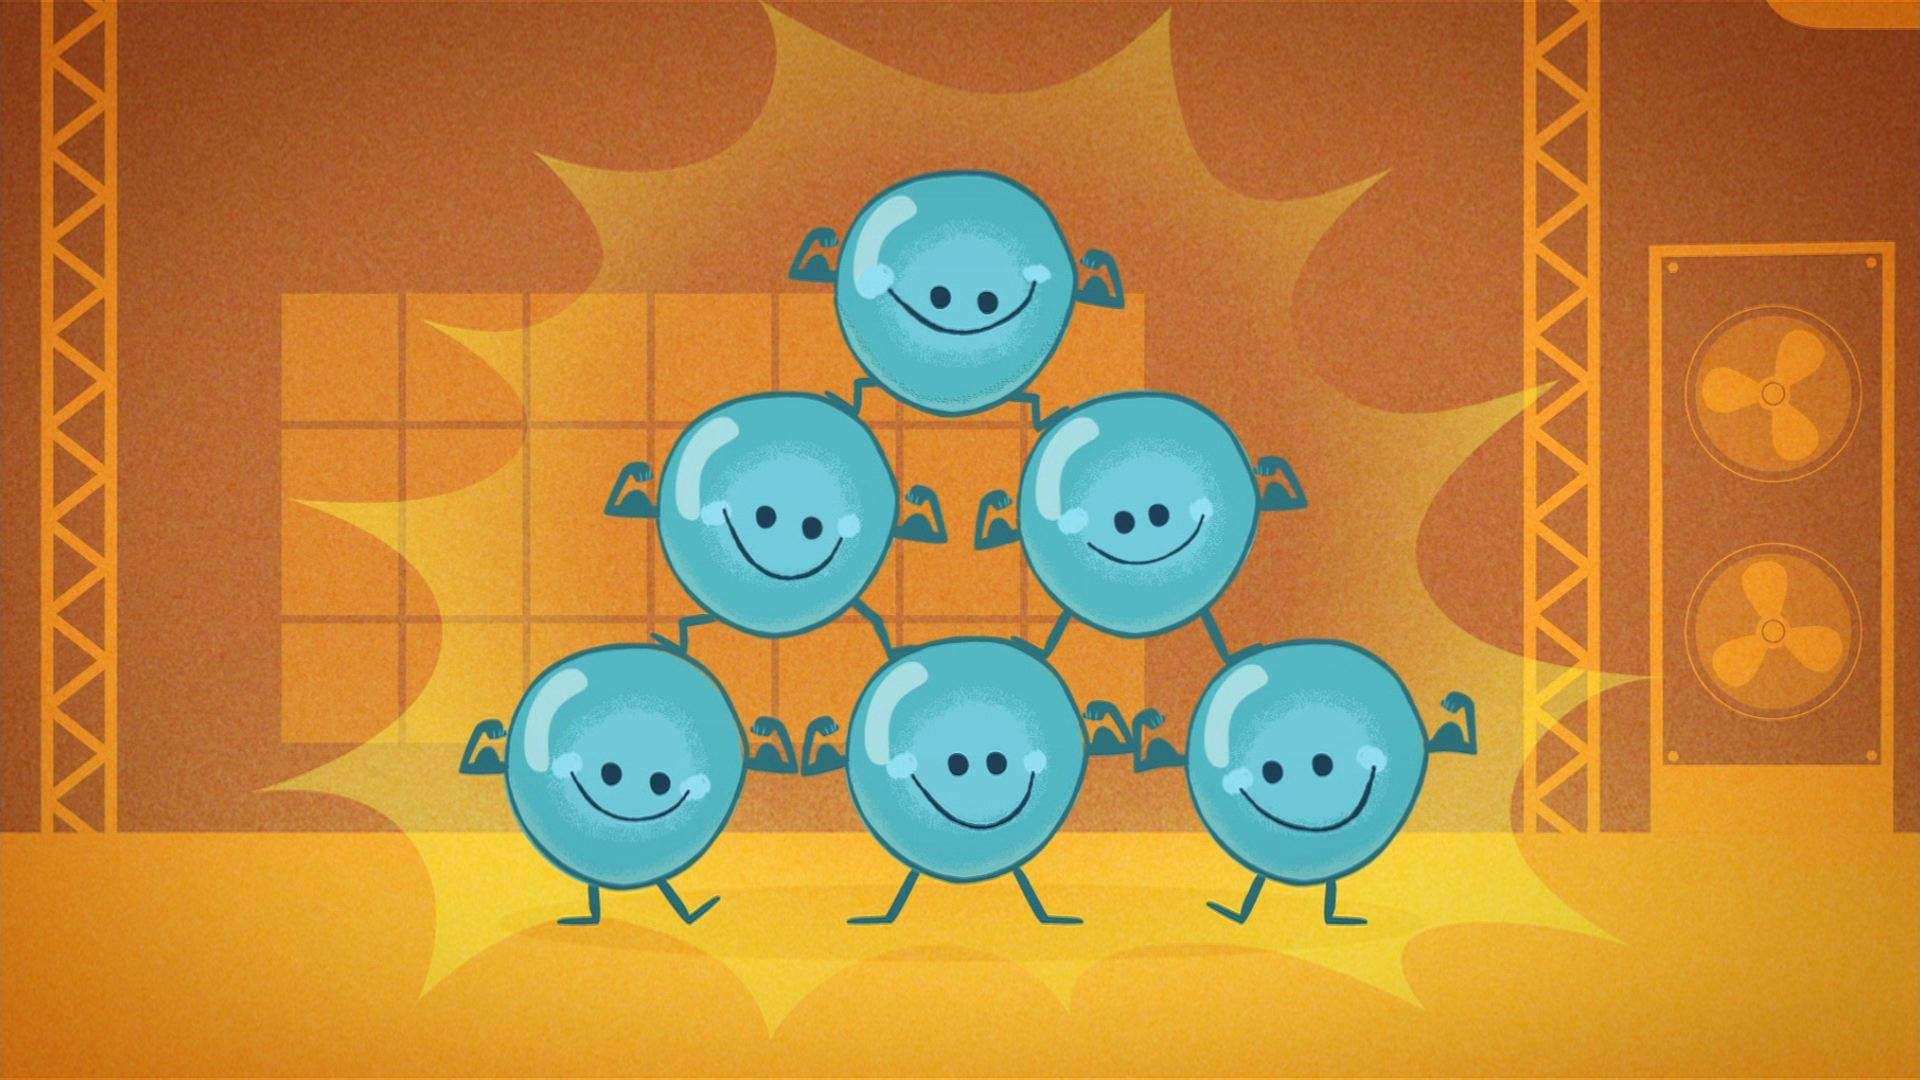
\includegraphics[width=15cm]{./images/cellule.jpg}~\\[3cm]

      \HRule \\[0.5cm]
      \textsc{\LARGE \doctitle \\[0.5cm]}
      \textbf{\Large Manuel d'utilisation \\[0.5cm]}
      \HRule \\[1.0cm]

		\docauthor
      ~\\[1.0cm]
      \today

      \vfill{}
      
    \end{center}
  \end{titlepage}



\shorttoc{Sommaire}{2}

\setcounter{page}{1}

\newpage
	

  \section{Présentation du logiciel}
	
	Madjan est un logiciel simulation d'automate cellulaire  adapté du jeux de la vie\footnote{inventé par \name{John Horton Conway} en 1970}. Cette adaptation comme le "jeu" d'origine n'est pas à proprement parlé un jeux vidéo mais un  automate  cellulaire définie sur une grille carrée a deux dimensions. Les cellules de la grille contiennent des pions qui naitront ou mourront durant les différentes générations. L'utilisateur n'aura aucune interaction durant le processus du jeux sauf pour le lancement et le paramétrage.
 	La distinction de cette adaption se fait dans le comportement qui est définie à l'aide de plugins\footnote{module chargé dynamiquement durant l'éxécution}. 
    Cette application permet, en fonction d'un paramétrage adéquate,de modéliser de nombreux processus tels que la propagation d'un incendie de fôret, dissémination de virus, etc\dots 
    
  \newpage  
  \section{Installation}
  Notre application est multi-plateforme  vous trouverez ci-dessous les différents moyens pour lancer l'application \textbf{Madjan} en fonction de votre système d'exploitation.
  
  	\subsection{Prérequis}
  Pour pouvoir compiler l'application \emph{Madjan} il est nécessaire qu'il soit installé sur votre poste \textbf{QT 4.8} disponible à cette adresse \hyperref[http://download.qt-project.org/archive/qt/4.8/]{QT4.8}. Vous pouvez choisir n'importe quelle version (de la 4.8.0 à la 4.8.6).
   La compilation sur  le système d'exploitation Windows n'est pas nécessaire un executable est déjà présent, voir chapitre \ref{execWind}. Cependant pour les utilisateurs avancés il est possible de  recompiler l'application, voir chapitre \ref{compilWind}.
   
  	\subsection{Compilation}
    
    	 \subsubsection{Compilation sous Mac et linux}
    	 	Un script d'installation destiné à la compilation de l'application est présent dans le dossier source Madjan.\\ 
            Pour l'exécuter:
           \begin{itemize}
           	 \item Ouvrez un terminal.
             \item Placez-vous dans le dossier \emph{madjan/}.
             \item Lancez le script install.sh : \$./install.sh
           \end{itemize}
           
   		 \subsubsection{Compilation sous Windows}\label{compilWind}
     Pour recompiler l'application sous le système d'exploitation  Windows il vous faut installer \emph{gnu-make} disponible à cette adresse : \hyperref[http://gnuwin32.sourceforge.net/packages/make.htm]{gnu-make}. Ainsi que \emph{qt-creator} disponible à cette adresse: \hyperref[http://sourceforge.net/projects/qtcreator.mirror/]{qt-creator}. Ensuite il vous faudra configurer \emph{qt-creator} pour recevoir le projet en utilisant madjan.pro se trouvant le dossier src/.
A noter que ce le fichier madjan.pro est partager par les différents système d'exploitation, il vous faudra sous Windows copier les dossiers de plugins directement dans le dossier de plugins présent dans le dossier de  compilation.
     \newpage
	\subsection{Exécution}
    Après la compilation du programme un exécutable permettant de lancer l'application sera disponible en fonction du système d'exploitation que vous utilisez. A noter que pour windows il n'est pas nécessaire de compiler l'application.
    
         \subsubsection{Exécution sous Linux}
          Dans le dossier source de l'application Madjan vous pouvez lancer l'application soit en passant par un gestionnaire de fichier et en double cliquant sur l'exécutable nommer "Madjan"  soit  l'aide d'un terminale, vous placez dans le dossier source et lancez l'exécutable. 
          
         \subsubsection{Exécution sous Mac}
    	 	Dans le dossier source de l'application Madjan vous pouvez lancer l'application soit en passant par un gestionnaire de fichier et en double cliquant sur l'exécutable nommer "Madjan.app"  soit  l'aide d'un terminale, vous placez dans le dossier source et lancez l'exécutable.
            
    	\subsubsection{Exécution sous Windows}\label{execWind}
       Pour lancer l'application un exécutable madjan.exe est disponible dans le dossier /bin-windows/release/ de l'application.
  
    \newpage
  \section{Utilisation}
  	
    
    \subsection{Règles}
     
    La simulation de l'automate cellulaire suit différentes règles qui peuvent être paramétrées par un plugin:
    
     \subsubsection{Propagation}\label{prop}
     
     	La propagation est un élément clé de l'application, elle permet de désigner la façon dont les cellules meurent, naissent etc\dots \\
    	Par défaut l'application propose une propagation pour une cellule  qui se base sur son nombre de cellules voisines (dans notre cas 8 comme sur la figure \ref{fig:voisinPion}).
        

	   
      	\begin{figure}[htb]
        	\begin{center}
        	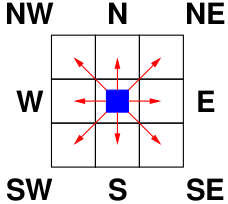
\includegraphics[width=0.3\textwidth]{./images/cells-voisines.png}\caption{\label{fig:voisinPion}les 8 voisins d'un pion}
             \end{center}
      	\end{figure}
      	
      	\FloatBarrier

   On peut voir sur le tableau \ref{tab:etatPion} les états possibles d'un pion en fonction de ses voisins d'une génération $n$ à une génération $n+1$ 
       
        
       \begin{table}[htb]
         \begin{center}
  			\begin{tabular}{  | c | c | }
    		\hline
     		\rowcolor{blue!20}\textbf{nombre de voisin génération $n$} & \textbf{destinée génération $n+1$} \\   
         	 \hline
     		  moin de 2 & meurt de solitude   \\ 
        	 \hline
     		  plus de 3 & meurt de surpopulation  \\
	 	     \hline
          	  3	& survit \\
          	 \hline
   			\end{tabular}      
            \caption{\label{tab:etatPion}tableau de la destinée d'un pion en fonction du nombre de voisin}
           \end{center}
        \end{table}
        
 		Une dernière règle subsiste, celle où une cellule ne contient pas de pion mais possède au moins 2 voisins il y à alors la naissance d'un pion.

      \subsubsection{Type des pions}
      
      Les pions actifs sont tous par défaut de type "vivant", dans ce cas ils sont en cour de vie. Dans le cas où il n'y a pas de pion visible dans une cellule de la grille, un pion inactif existe tout de même mais est typé "Empty"(vide). 
      D'autres types de pions peuvent être définis pour représenter des états intermédiaires des pions: 
      
       \begin{itemize}
	       \item naissant : pion naissant
		   \item mourrant : pion mourant
	       \item \dots
       \end{itemize}
       
	Ces définitions restent des exemples de types de pion et peuvent être définis à l'aide de \hyperref[plugin]{plugins}.\\
    Seul le type de pion "Empty" qui est un pion inactif ne peut être modifié.
	
     \subsection{Interface}
     
      Dès lors que vous avez lancez l'exécutable de l'application \emph{Madjan}, vous vous retrouverez face à l'interface utilisateur ou vous aurez la possiblité de configurer l'application, de lancer la simulation, etc\dots
      
      \subsubsection{Choix du plugin}
     Un bouton nommé \emph{Plugins} vous permet d'afficher la liste des plugins disponibles et d'en sélectionner un en cliquant sur le plugin souhaité. L'application suivra les paramètres définies par le plugin choisi.
     
     \newpage
     \subsubsection{Choix de la taille de la grille}
     
     Deux cases \emph{Height} (hauteur) et \emph{Width} (largeur) vous permettrons de définir la taille initiale de votre grille. Pour appliquer les paramètres de cette grille, vous devrez cliquez sur le bouton \emph{Apply} (appliquer) se trouvant à droite des cases.\\
     
    \begin{figure}[htb]
        	\begin{center}
        	
\includegraphics[width=0.8\textwidth]{./images/tailleGrille.png}\caption{\label{fig:tailleGrille} cases de définition des tailles de la grille}
             \end{center}
      	\end{figure}
      	
      	\FloatBarrier
    
    Si vous souhaitez changer la taille de votre grille durant le déroulement de la simulation, vous pouvez redéfinir les champs \emph{Width} et \emph{Height} et appliquer cette nouvelle configuration de grille avec le bouton \emph{Apply}. \\ A noter que les pions seront réinitialisés mais que la simulation sera toujours en cour tant que vous n'aurez pas appuyé sur le bouton \emph{Pause}.
    	\newpage
        \subsubsection{Placer les pions soit même}
        
    Il est possible de choisir le positionnement des différents pions avant de lancer la simulation. Pour ce faire, une liste des différents types de pion disponibles est présente à gauche de la grille.    
    Vous pourrez alors cliquer sur un des types de pion et choisir la cellule de la grille dans laquelle vous souhaitez le mettre.
    
		\begin{figure}[htb]
        	\begin{center}
        	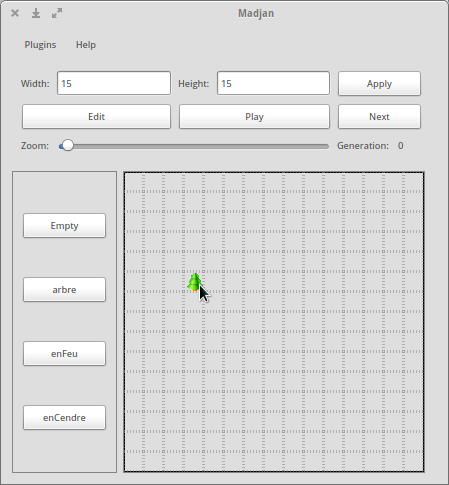
\includegraphics[width=0.8\textwidth]{./images/placementPion.png}\caption{\label{fig:placementPion} placement d'un pion de type "arbre" dans la grille}
             \end{center}
      	\end{figure}
      	
      	\FloatBarrier
        
     Dans cette exemple nous ajoutons un pion de type arbre dans une cellule de la grille après avoir cliqué à gauche sur le bouton correspondant à ce type de pion.
    	\newpage
 		\subsubsection{Placer les pions aléatoirement}
        
     Si vous ne souhaitez pas définir  l'emplacement de vos pions un par un dans la grille vous pouvez choisir une disposition générée aléatoirement dans la grille.
     Pour pouvoir utiliser cette fonction  vous pouvez cliquer sur le bouton \emph{edit} (edition). Ce dernier vous ouvrira une fenêtre où deux colonnes sont présentent, la colonne \emph{Création} où vous serons demandés les paramètres de création de la grille aléatoire et la colonne \emph{Stop Conditions} où vous pourrez indiquer si vous le souhaitez des paramètres d'arrêt de la simulation.
     Les paramètres \emph{Width} et \emph{Height} vous permettrons d'indiquer la taille de la grille souhaitée.
     Les autres paramètres correspondent aux pourcentages de pions attendu sur la grille dans la colonne \emph{Creation} et aux pourcentages de pions pour lesquels la simulation s'arrête dans la colonne \emph{Stop Conditions}.\\
     
    Attention Les pourcentages sont à indiquer sans le symbole de pourcentage \%. Pour les pourcentages de la colonne \emph{Stop Conditions} les pourcentages doivent être précédé d'un signe inférieur  "\textless" ou un signe supérieur "\textgreater" pour indiquer une conditions d'arrêt supérieur ou égale ou inférieur ou égale au pourcentage indiqué. 
    
     	\begin{figure}[htb]
        	\begin{center}
        	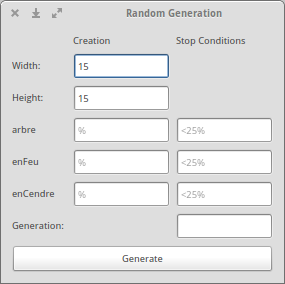
\includegraphics[width=0.6\textwidth]{./images/randomWindow.png}\caption{\label{fig:randomWindow} fenêtre de la configuration de la génération aléatoire}
             \end{center}
      	\end{figure}
        \FloatBarrier
  Pour lancer la génération aléatoire de la grille il vous suffira, après avoir indiqué les différents paramètres, d'appuyer sur le bouton \emph{Generate}.
        \newpage
     	\subsubsection{Gestion de la simulation}
    Pour pouvoir agir sur la simulation tel que le lancement ou la mise en pause, voici la liste des commandes disponibles : 
   		\begin{itemize}
        	\item Bouton \emph{Play} : lance une simulation continue de toutes les étapes de génération qui sont exécutées à la suite. Ce bouton est remplacé par le bouton Pause.
            \item Bouton \emph{Pause}: met en pause la simulation. Ce bouton est remplacé par le bouton Play 
            \item Bouton \emph{Next}: simule la génération suivante et permet d'avoir chaque itération de la simulation.
            \item \emph{Zoom}: cette commande permet d'agrandir ou de réduire la grille, de gauche à droite la commande agrandie la grille et de droite à gauche réduit la grille. \\
        \end{itemize}
 A noter qu'il y a la présence d'un indicateur \emph{Génération} qui permet de savoir à quelle génération
se trouve la simulation.  

	\newpage
  	 \section{Plugins}\label{plugin}
   
   	 Les plugins vont vous permettre de définir vous même les différents comportements de l'application. Les plugins disponibles sont au format \emph{XML} disponible dans le dossier \commande{/plugins}.
     
		\subsection{Plugins disponibles}
		
       Par défaut l'application dispose de trois plugins disponibles dans le dossier plugin de cette dernière.
       
       \subsubsection{Plugins du jeux de la vie}
       
 	Ce plugin par défaut configure l'application avec des règles de propagations présentent dans le \hyperref[prop]{chapitre \ref{prop}} ainsi qu'un type de pion qui est de type "vivant" et qui en fonction des règles de propagations se transforme en type "Empty" ou reste de type "vivant".
    

      \subsubsection{Plugin de feu de forêt }
    Ce plugin a pour but de présenter la propagation d'un feu de forêt en fonction des conbustibles présents, en l'occurrence des arbres.\\
    Les types de pions disponibles sont : 
    
    	\begin{itemize}
        	\item arbre : ce pion représente le conbustible. 
            \item enCendre : ce pion représente l'état en cendre.
            \item enFeu: ce pion représente l'état en feu d'un arbre. \\
        \end{itemize} 
   Ces pions sont représentés par des images :
    
        \begin{itemize}
        	\item arbre : image d'un arbre vert.
            \item enCendre : image d'un arbre en cendre.
            \item enFeu: image d'un arbre en feu.
        \end{itemize} 
        
    Les règles de propagations sont simples, si un pion de type "arbre" a un voisin de type "enFeu" à la prochaine génération il deviendra un pion de type "enFeu". A la génération suivante il deviendra un pion de type "enCendre".  
    \newpage
       \subsubsection{Plugin de "super" feu de forêt }
    Ce plugin a pour but de présenter la propagation d'un feu de forêt en fonction des conbustibles présent, en l'occurrence des arbres. En comparaison avec la version simple un type de pion intermédiaire a été rajouté. \\
    Les types de pions disponibles sont : 
    
    	\begin{itemize}
        	\item Arbre : ce pion représente le conbustible 
            \item Arbre en cendre : ce pion représente l'état en cendre.
            \item Arbre en feu: ce pion représente l'état en feu d'un arbre .
            \item  Arbre en Cendre: ce pion représente l'état en départ de feu d'un arbre.\\
        \end{itemize} 
        
\noindent Ces pions sont représentés par des images:
    
        \begin{itemize}
        	\item arbre : image d'un arbre vert.
            \item enCendre : image d'un arbre en cendre.
            \item enFeu: image d'un arbre en feu.
            \item enPetitFeu: image d'un arbre en départ de feu.\\
        \end{itemize} 
        
\noindent  Les règles de propagations sont les suivantes : 
  
        \begin{itemize}
        	\item si un arbre a plus de deux voisins de type  arbre en départ de feu il devient un abre en départ de feu.
            \item si un arbre a plus de quatre voisins de type arbre en départ de feu il devient un arbre en feu. 
            \item si un arbre a un ou plus de un voisin de type  en feu il devient en feu. 
            \item un arbre de type en départ de feu deviendra de type en feu.
			\item un arbre de type en feu deviendra de type en cendre.
			\end{itemize} 
        
        \newpage
       \subsection{Charger son plugins}
       
      Si vous souhaitez crée votre propre plugin pour définir vos propres caractéristiques des jetons (images, comportements, etc\dots), vous pouvez ajouté un plugin à la racine du projet dans le dossier \commande{plugins/} qui se trouve au même niveau que le dossier \commande{src/}. Dans le dossier \commande{plugins/} vous pourrez définir n'importe quel nom de dossier qui contiendra  que le fichier \commande{plugin.xml} et si vous le souhaitez le dossier source d'images pour les pions.
      
      
      \subsection{Règles de création d'un plugin}
      
     Pour crée un plugin différentes balises peuvent être intégrées dans un fichier nommé \commande{plugin.xml} :
     	
        \subsubsection{Balises recommandées}
        
        Certaines balises sont recommandées pour respecter la structure d'un plugin :
        \begin{enumerate}
        	\item \balise{plugin}{\dots}: la balise racine du document xml où toutes règles seront indiqués dedans.
        	\item \balise{name}{un nom unique} : le nom du plugin apparaissant dans l'interface utilisateur (obligatoire).         
            \item \balise{description}{une description} : description du plugin(optionelle)
            \item \balise{version}{la version}: version du plugin (optionelle)
         	\item \balise{cellBackground}{fondDuneCellule.format}: le nom du fichier image de fond d'une cellule
        \end{enumerate}
        

         \subsubsection{Les pions}
         	Vous pouvez définir les règles de vos pions à l'aide des balises suivantes : 
 
            	\begin{itemize}
                  \item \balise{pawns}{\dots} : balise où seront présents le ou les pions et la ou leurs propriétés :
                	\begin{itemize}
                		\item \balise{pawn}{\dots}: balise où seront présentent les propriétés du pions : 			  
                        \begin{itemize}
                        \item \balise{id}{un id unique}: id du pion qui doit être unique
               			\item \balise{name}{un nom}: le nom du pion
                		\item \balise{icon}{image.format}: l'icon au format d'une image du pion. (attention à ne pas mettre de \slash devant le nom du répertoire ou de l'image)
  		       		  \end{itemize}	
                    \end{itemize} 
               \end{itemize}
               
        Plusieurs balises \emph{pawn}(pion) peuvent être définies avec leurs propriétés seulement si les identifiants sont différents sinon l'application ne prendra pas en compte les pions qui partage le même identifiant.
        
       
		 \subsubsection{Les Règles de propagations associés au pions}
         
         Les règles de propagations peuvent être écrite en lien directe avec les pions définis dans le fichier \commande{plugin.xml}. Pour en écrire de nouvelles vous pouvez utiliser les balises suivantes: 
         
         	\begin{itemize}
            \item \balise{rules}{\dots} : balise qui contient la ou les règles associés aux pions : \\				
            	\begin{itemize}
                	\item \bwithparam{rule}{ pawn="nom de l'état du pion" newPawn="nom du nouveau pion crée"}{\dots} \\: balise permettant de définir le nouveau pion (\emph{newPawn}) qui sera généré à la place du pion (\emph{pawn}) en fonction des règles appliquées :\\ 
                    	\begin{itemize}
                              \item \bwithparam{pawnNumberIsEqual}{ pawn="nom du pion"}{nombre de pion voisin}: \\ balise qui définie une conditions permetant à un pion d'être transformé, à la génération suivante, si le nombre de type de pion \emph{pawn} est \textbf{égale} au \emph{nombre de pion} voisin indiqué.
                              \item \bwithparam{pawnNumberIsLower}{ pawn="nom du pion"}{nombre de pion voisin}: \\ balise qui définie une conditions permetant à un pion d'être transformé, à la génération suivante, si le nombre de type de pion \emph{pawn} est \textbf{inférieur} au \emph{nombre de pion} voisin indiqué.		
                             \item \bwithparam{pawnNumberIsGreater}{ pawn="nom du pion"}{nombre de pion voisin}: \\ balise qui définie une conditions permetant à un pion d'être transformé, à la génération suivante, si le nombre de type de pion \emph{pawn} est \textbf{supérieur} au \emph{nombre de pion} voisin indiqué.
                        \end{itemize}
                \end{itemize}
         	
        	\end{itemize}
    \newpage
    
Comme pour les pions il est possible de définir plusieurs règles de propagations avec leurs conditions d'exécutions.\\ 
Dans le cas ou plusieurs règles sont appliqués pour le même pions seul celle ou le pion satifsait les conditions sera exécutée (utilisation du booléen OU). Enfin pour qu'une règle soit appliquée, le pion doit satisfaire toutes les conditions de cette dernière.\\ 

Attention à ne pas définir des conditions contradictoires tels qu'un nombre de voisin supérieur et inférieur, dans un tel cas la règle contenant ces conditions ne sera pas appliquée. \\ 

En outre si deux règles définies, pour un pion, possèdent les mêmes conditions mais pas le même nombre de voisin pour satisfaire la ou les conditions alors la dernière règle sera exécutée.
\newpage


\addcontentsline{toc}{section}{Table des matières}
\tableofcontents

 
    
     
\end{document}